\documentclass{beamer}

\usetheme[coloredtitles, coloredblocks]{vub}
\usepackage{amsmath,amsfonts,amsthm,amssymb,mathtools}
\usepackage{graphicx}
% \usepackage[shortlabels]{enumitem}
% \usepackage{hyperref}
% \usepackage{cleveref}
\usepackage{tikz-cd}

% %% PACKAGES

\usepackage{amsmath,amsfonts,amsthm,amssymb,mathtools}
\usepackage[shortlabels]{enumitem}
\usepackage{hyperref}
\usepackage{cleveref}
\usepackage{tikz-cd}

%% Theorem environments
\theoremstyle{plain}
\newtheorem{theorem}{Theorem}[section]
\newtheorem{lemma}[theorem]{Lemma}
\newtheorem{prop}[theorem]{Proposition}
\newtheorem{corollary}[theorem]{Corollary}
\newtheorem*{theorem*}{Theorem}
\newtheorem*{lemma*}{Lemma}
\newtheorem*{prop*}{Proposition}
\newtheorem*{corollary*}{Corollary}

\theoremstyle{definition}
\newtheorem{definition}[theorem]{Definition}
\newtheorem{example}[theorem]{Example}
\newtheorem{exercise}[theorem]{Exercise}
\newtheorem*{definition*}{Definition}
\newtheorem*{example*}{Example}
\newtheorem*{exercise*}{Exercise}

\theoremstyle{remark}
\newtheorem{remark}[theorem]{Remark}
\newtheorem*{remark*}{Remark}

%===========================================================%
%The code below customises theorem numbering
%===========================================================%

\theoremstyle{plain}
\newtheorem{innercustomgenericplain}{\customgenericname}
\providecommand{\customgenericname}{}
\newcommand{\newcustomtheoremplain}[2]{%
    \crefname{#2}{#2}{#2s}%
    \newenvironment{#1}[1]
    {%
        \renewcommand\customgenericname{#2}%
        \crefalias{innercustomgenericplain}{#2}%
        \renewcommand\theinnercustomgenericplain{##1}%
        \innercustomgenericplain
    }
    {\endinnercustomgenericplain}
}

\theoremstyle{definition}
\newtheorem{innercustomgenericdefinition}{\customgenericname}
\providecommand{\customgenericname}{}
\newcommand{\newcustomtheoremdefinition}[2]{%
    \crefname{#2}{#2}{#2s}%
    \newenvironment{#1}[1]
    {%
        \renewcommand\customgenericname{#2}%
        \crefalias{innercustomgenericdefinition}{#2}%
        \renewcommand\theinnercustomgenericdefinition{##1}%
        \innercustomgenericdefinition
    }
    {\endinnercustomgenericdefinition}
}

\theoremstyle{remark}
\newtheorem{innercustomgenericremark}{\customgenericname}
\providecommand{\customgenericname}{}
\newcommand{\newcustomtheoremremark}[2]{%
    \crefname{#2}{#2}{#2s}%
    \newenvironment{#1}[1]
    {%
        \renewcommand\customgenericname{#2}%
        \crefalias{innercustomgenericremark}{#2}%
        \renewcommand\theinnercustomgenericremark{##1}%
        \innercustomgenericremark
    }
    {\endinnercustomgenericremark}
}


\newcustomtheoremplain{customtheorem}{Theorem}
\newcustomtheoremplain{customlemma}{Lemma}
\newcustomtheoremplain{customprop}{Proposition}
\newcustomtheoremplain{customcorollary}{Corollary}

\newcustomtheoremdefinition{customdefinition}{Definition}
\newcustomtheoremdefinition{customexample}{Example}
\newcustomtheoremdefinition{customexercise}{Exercise}

\newcustomtheoremremark{customremark}{Remark}

\newcommand{\inv}{^{-1}}
\newcommand{\defeq}{\overset{\mathrm{def}}{=}}


\newcommand{\liff}{\leftrightarrow}
\newcommand{\lthen}{\rightarrow}
\newcommand{\opname}{\operatorname}
\newcommand{\surjto}{\twoheadrightarrow}
\newcommand{\injto}{\hookrightarrow}
\DeclareMathOperator{\img}{im} % Image
\DeclareMathOperator{\Img}{Im} % Image
\DeclareMathOperator{\coker}{coker} % Cokernel
\DeclareMathOperator{\Coker}{Coker} % Cokernel
\DeclareMathOperator{\Ker}{Ker} % Kernel
\DeclareMathOperator{\rank}{rank} % rank
\DeclareMathOperator{\Spec}{Spec} % spectrum
\DeclareMathOperator{\Tr}{Tr} % trace
\DeclareMathOperator{\pr}{pr} % projection
\DeclareMathOperator{\ext}{ext} % extension
\DeclareMathOperator{\pred}{pred} % predecessor
\DeclareMathOperator{\dom}{dom} % domain
\DeclareMathOperator{\cod}{cod} % codomain
\DeclareMathOperator{\ran}{ran} % range
\DeclareMathOperator{\Hom}{Hom} % homomorphism
\DeclareMathOperator{\Mor}{Mor} % morphisms
\DeclareMathOperator{\ob}{ob} % objects
\DeclareMathOperator{\mor}{mor} % morphisms
\DeclareMathOperator{\Fun}{Fun} % functors
\DeclareMathOperator{\Nat}{Nat} % natural transformations
\DeclareMathOperator{\End}{End} % endomorphism
\DeclareMathOperator{\Ann}{Ann} % annihilator

% Category Theory
\DeclareMathOperator{\Mod}{\mathbf{Mod}}
\DeclareMathOperator{\Top}{\mathbf{Top}}
\DeclareMathOperator{\Vect}{\mathbf{Vect}}
\DeclareMathOperator{\Ring}{\mathbf{Ring}}
\DeclareMathOperator{\Rng}{\mathbf{Rng}}
\DeclareMathOperator{\Ab}{\mathbf{Ab}}
\DeclareMathOperator{\Set}{\mathbf{Set}}
\DeclareMathOperator{\Sh}{\mathbf{Sh}}
\DeclareMathOperator{\PSh}{\mathbf{PSh}}

\newcommand{\ol}{\overline}
\newcommand{\ul}{\underline}
\newcommand{\wt}{\widetilde}
\newcommand{\wh}{\widehat}
\newcommand{\norm}[1]{\left\| #1 \right\|}
\newcommand{\inner}[2]{\left\langle #1 , #2 \right\rangle}


% Things Lie
\newcommand{\kb}{\mathfrak b}
\newcommand{\kg}{\mathfrak g}
\newcommand{\kh}{\mathfrak h}
\newcommand{\kn}{\mathfrak n}
\newcommand{\ku}{\mathfrak u}
\newcommand{\kz}{\mathfrak z}
\DeclareMathOperator{\Ext}{Ext} % Ext functor
\DeclareMathOperator{\Tor}{Tor} % Tor functor
\newcommand{\gl}{\opname{\mathfrak{gl}}} % frak gl group
\renewcommand{\sl}{\opname{\mathfrak{sl}}} % frak sl group chktex 6

% More script letters etc.
\newcommand{\SA}{\mathcal A}
\newcommand{\SB}{\mathcal B}
\newcommand{\SC}{\mathcal C}
\newcommand{\SF}{\mathcal F}
\newcommand{\SG}{\mathcal G}
\newcommand{\SH}{\mathcal H}
\newcommand{\OO}{\mathcal O}

\newcommand{\SCA}{\mathscr A}
\newcommand{\SCB}{\mathscr B}
\newcommand{\SCC}{\mathscr C}
\newcommand{\SCD}{\mathscr D}
\newcommand{\SCE}{\mathscr E}
\newcommand{\SCF}{\mathscr F}
\newcommand{\SCG}{\mathscr G}
\newcommand{\SCH}{\mathscr H}

% Mathfrak primes
\newcommand{\km}{\mathfrak m}
\newcommand{\kp}{\mathfrak p}
\newcommand{\kq}{\mathfrak q}

% number sets
\newcommand{\RR}[1][]{\ensuremath{\ifstrempty{#1}{\mathbb{R}}{\mathbb{R}^{#1}}}}
\newcommand{\NN}[1][]{\ensuremath{\ifstrempty{#1}{\mathbb{N}}{\mathbb{N}^{#1}}}}
\newcommand{\ZZ}[1][]{\ensuremath{\ifstrempty{#1}{\mathbb{Z}}{\mathbb{Z}^{#1}}}}
\newcommand{\QQ}[1][]{\ensuremath{\ifstrempty{#1}{\mathbb{Q}}{\mathbb{Q}^{#1}}}}
\newcommand{\CC}[1][]{\ensuremath{\ifstrempty{#1}{\mathbb{C}}{\mathbb{C}^{#1}}}}
\newcommand{\PP}[1][]{\ensuremath{\ifstrempty{#1}{\mathbb{P}}{\mathbb{P}^{#1}}}}
\newcommand{\HH}[1][]{\ensuremath{\ifstrempty{#1}{\mathbb{H}}{\mathbb{H}^{#1}}}}
\newcommand{\FF}[1][]{\ensuremath{\ifstrempty{#1}{\mathbb{F}}{\mathbb{F}^{#1}}}}
% expected value
\newcommand{\EE}{\ensuremath{\mathbb{E}}}
\newcommand{\charin}{\text{ char }}
\DeclareMathOperator{\sign}{sign}
\DeclareMathOperator{\Aut}{Aut}
\DeclareMathOperator{\Inn}{Inn}
\DeclareMathOperator{\Syl}{Syl}
\DeclareMathOperator{\Gal}{Gal}
\DeclareMathOperator{\GL}{GL} % General linear group
\DeclareMathOperator{\SL}{SL} % Special linear group

%---------------------------------------
% BlackBoard Math Fonts :-
%---------------------------------------

%Captital Letters
\newcommand{\bbA}{\mathbb{A}}	\newcommand{\bbB}{\mathbb{B}}
\newcommand{\bbC}{\mathbb{C}}	\newcommand{\bbD}{\mathbb{D}}
\newcommand{\bbE}{\mathbb{E}}	\newcommand{\bbF}{\mathbb{F}}
\newcommand{\bbG}{\mathbb{G}}	\newcommand{\bbH}{\mathbb{H}}
\newcommand{\bbI}{\mathbb{I}}	\newcommand{\bbJ}{\mathbb{J}}
\newcommand{\bbK}{\mathbb{K}}	\newcommand{\bbL}{\mathbb{L}}
\newcommand{\bbM}{\mathbb{M}}	\newcommand{\bbN}{\mathbb{N}}
\newcommand{\bbO}{\mathbb{O}}	\newcommand{\bbP}{\mathbb{P}}
\newcommand{\bbQ}{\mathbb{Q}}	\newcommand{\bbR}{\mathbb{R}}
\newcommand{\bbS}{\mathbb{S}}	\newcommand{\bbT}{\mathbb{T}}
\newcommand{\bbU}{\mathbb{U}}	\newcommand{\bbV}{\mathbb{V}}
\newcommand{\bbW}{\mathbb{W}}	\newcommand{\bbX}{\mathbb{X}}
\newcommand{\bbY}{\mathbb{Y}}	\newcommand{\bbZ}{\mathbb{Z}}

%---------------------------------------
% MathCal Fonts :-
%---------------------------------------

%Captital Letters
\newcommand{\mcA}{\mathcal{A}}	\newcommand{\mcB}{\mathcal{B}}
\newcommand{\mcC}{\mathcal{C}}	\newcommand{\mcD}{\mathcal{D}}
\newcommand{\mcE}{\mathcal{E}}	\newcommand{\mcF}{\mathcal{F}}
\newcommand{\mcG}{\mathcal{G}}	\newcommand{\mcH}{\mathcal{H}}
\newcommand{\mcI}{\mathcal{I}}	\newcommand{\mcJ}{\mathcal{J}}
\newcommand{\mcK}{\mathcal{K}}	\newcommand{\mcL}{\mathcal{L}}
\newcommand{\mcM}{\mathcal{M}}	\newcommand{\mcN}{\mathcal{N}}
\newcommand{\mcO}{\mathcal{O}}	\newcommand{\mcP}{\mathcal{P}}
\newcommand{\mcQ}{\mathcal{Q}}	\newcommand{\mcR}{\mathcal{R}}
\newcommand{\mcS}{\mathcal{S}}	\newcommand{\mcT}{\mathcal{T}}
\newcommand{\mcU}{\mathcal{U}}	\newcommand{\mcV}{\mathcal{V}}
\newcommand{\mcW}{\mathcal{W}}	\newcommand{\mcX}{\mathcal{X}}
\newcommand{\mcY}{\mathcal{Y}}	\newcommand{\mcZ}{\mathcal{Z}}


%---------------------------------------
% Bold Math Fonts :-
%---------------------------------------

%Captital Letters
\newcommand{\bmA}{\boldsymbol{A}}	\newcommand{\bmB}{\boldsymbol{B}}
\newcommand{\bmC}{\boldsymbol{C}}	\newcommand{\bmD}{\boldsymbol{D}}
\newcommand{\bmE}{\boldsymbol{E}}	\newcommand{\bmF}{\boldsymbol{F}}
\newcommand{\bmG}{\boldsymbol{G}}	\newcommand{\bmH}{\boldsymbol{H}}
\newcommand{\bmI}{\boldsymbol{I}}	\newcommand{\bmJ}{\boldsymbol{J}}
\newcommand{\bmK}{\boldsymbol{K}}	\newcommand{\bmL}{\boldsymbol{L}}
\newcommand{\bmM}{\boldsymbol{M}}	\newcommand{\bmN}{\boldsymbol{N}}
\newcommand{\bmO}{\boldsymbol{O}}	\newcommand{\bmP}{\boldsymbol{P}}
\newcommand{\bmQ}{\boldsymbol{Q}}	\newcommand{\bmR}{\boldsymbol{R}}
\newcommand{\bmS}{\boldsymbol{S}}	\newcommand{\bmT}{\boldsymbol{T}}
\newcommand{\bmU}{\boldsymbol{U}}	\newcommand{\bmV}{\boldsymbol{V}}
\newcommand{\bmW}{\boldsymbol{W}}	\newcommand{\bmX}{\boldsymbol{X}}
\newcommand{\bmY}{\boldsymbol{Y}}	\newcommand{\bmZ}{\boldsymbol{Z}}
%Small Letters
\newcommand{\bma}{\boldsymbol{a}}	\newcommand{\bmb}{\boldsymbol{b}}
\newcommand{\bmc}{\boldsymbol{c}}	\newcommand{\bmd}{\boldsymbol{d}}
\newcommand{\bme}{\boldsymbol{e}}	\newcommand{\bmf}{\boldsymbol{f}}
\newcommand{\bmg}{\boldsymbol{g}}	\newcommand{\bmh}{\boldsymbol{h}}
\newcommand{\bmi}{\boldsymbol{i}}	\newcommand{\bmj}{\boldsymbol{j}}
\newcommand{\bmk}{\boldsymbol{k}}	\newcommand{\bml}{\boldsymbol{l}}
\newcommand{\bmm}{\boldsymbol{m}}	\newcommand{\bmn}{\boldsymbol{n}}
\newcommand{\bmo}{\boldsymbol{o}}	\newcommand{\bmp}{\boldsymbol{p}}
\newcommand{\bmq}{\boldsymbol{q}}	\newcommand{\bmr}{\boldsymbol{r}}
\newcommand{\bms}{\boldsymbol{s}}	\newcommand{\bmt}{\boldsymbol{t}}
\newcommand{\bmu}{\boldsymbol{u}}	\newcommand{\bmv}{\boldsymbol{v}}
\newcommand{\bmw}{\boldsymbol{w}}	\newcommand{\bmx}{\boldsymbol{x}}
\newcommand{\bmy}{\boldsymbol{y}}	\newcommand{\bmz}{\boldsymbol{z}}

%---------------------------------------
% Scr Math Fonts :-
%---------------------------------------

\newcommand{\sA}{{\mathscr{A}}}   \newcommand{\sB}{{\mathscr{B}}}
\newcommand{\sC}{{\mathscr{C}}}   \newcommand{\sD}{{\mathscr{D}}}
\newcommand{\sE}{{\mathscr{E}}}   \newcommand{\sF}{{\mathscr{F}}}
\newcommand{\sG}{{\mathscr{G}}}   \newcommand{\sH}{{\mathscr{H}}}
\newcommand{\sI}{{\mathscr{I}}}   \newcommand{\sJ}{{\mathscr{J}}}
\newcommand{\sK}{{\mathscr{K}}}   \newcommand{\sL}{{\mathscr{L}}}
\newcommand{\sM}{{\mathscr{M}}}   \newcommand{\sN}{{\mathscr{N}}}
\newcommand{\sO}{{\mathscr{O}}}   \newcommand{\sP}{{\mathscr{P}}}
\newcommand{\sQ}{{\mathscr{Q}}}   \newcommand{\sR}{{\mathscr{R}}}
\newcommand{\sS}{{\mathscr{S}}}   \newcommand{\sT}{{\mathscr{T}}}
\newcommand{\sU}{{\mathscr{U}}}   \newcommand{\sV}{{\mathscr{V}}}
\newcommand{\sW}{{\mathscr{W}}}   \newcommand{\sX}{{\mathscr{X}}}
\newcommand{\sY}{{\mathscr{Y}}}   \newcommand{\sZ}{{\mathscr{Z}}}


%---------------------------------------
% Math Fraktur Font
%---------------------------------------

%Captital Letters
\newcommand{\mfA}{\mathfrak{A}}	\newcommand{\mfB}{\mathfrak{B}}
\newcommand{\mfC}{\mathfrak{C}}	\newcommand{\mfD}{\mathfrak{D}}
\newcommand{\mfE}{\mathfrak{E}}	\newcommand{\mfF}{\mathfrak{F}}
\newcommand{\mfG}{\mathfrak{G}}	\newcommand{\mfH}{\mathfrak{H}}
\newcommand{\mfI}{\mathfrak{I}}	\newcommand{\mfJ}{\mathfrak{J}}
\newcommand{\mfK}{\mathfrak{K}}	\newcommand{\mfL}{\mathfrak{L}}
\newcommand{\mfM}{\mathfrak{M}}	\newcommand{\mfN}{\mathfrak{N}}
\newcommand{\mfO}{\mathfrak{O}}	\newcommand{\mfP}{\mathfrak{P}}
\newcommand{\mfQ}{\mathfrak{Q}}	\newcommand{\mfR}{\mathfrak{R}}
\newcommand{\mfS}{\mathfrak{S}}	\newcommand{\mfT}{\mathfrak{T}}
\newcommand{\mfU}{\mathfrak{U}}	\newcommand{\mfV}{\mathfrak{V}}
\newcommand{\mfW}{\mathfrak{W}}	\newcommand{\mfX}{\mathfrak{X}}
\newcommand{\mfY}{\mathfrak{Y}}	\newcommand{\mfZ}{\mathfrak{Z}}
%Small Letters
\newcommand{\mfa}{\mathfrak{a}}	\newcommand{\mfb}{\mathfrak{b}}
\newcommand{\mfc}{\mathfrak{c}}	\newcommand{\mfd}{\mathfrak{d}}
\newcommand{\mfe}{\mathfrak{e}}	\newcommand{\mff}{\mathfrak{f}}
\newcommand{\mfg}{\mathfrak{g}}	\newcommand{\mfh}{\mathfrak{h}}
\newcommand{\mfi}{\mathfrak{i}}	\newcommand{\mfj}{\mathfrak{j}}
\newcommand{\mfk}{\mathfrak{k}}	\newcommand{\mfl}{\mathfrak{l}}
\newcommand{\mfm}{\mathfrak{m}}	\newcommand{\mfn}{\mathfrak{n}}
\newcommand{\mfo}{\mathfrak{o}}	\newcommand{\mfp}{\mathfrak{p}}
\newcommand{\mfq}{\mathfrak{q}}	\newcommand{\mfr}{\mathfrak{r}}
\newcommand{\mfs}{\mathfrak{s}}	\newcommand{\mft}{\mathfrak{t}}
\newcommand{\mfu}{\mathfrak{u}}	\newcommand{\mfv}{\mathfrak{v}}
\newcommand{\mfw}{\mathfrak{w}}	\newcommand{\mfx}{\mathfrak{x}}
\newcommand{\mfy}{\mathfrak{y}}	\newcommand{\mfz}{\mathfrak{z}}


\newtheorem{proposition}{Proposition}

% \usepackage[width=400pt]{geometry}

\DeclareMathOperator{\Open}{\mathbf{Open}}
\DeclareMathOperator{\opp}{opp}
\DeclareMathOperator{\Cont}{Cont}
\DeclareMathOperator{\Cov}{Cov}
\DeclareMathOperator{\colim}{colim}
\DeclareMathOperator{\id}{id}

\title{A Fluid Introduction to Condensed Mathematics}
\author{Wannes Malfait}
\date{}

\begin{document}
\maketitle

\begin{frame}
    \frametitle{Motivation}

    \textbf{Problem}: Algebra and topology clash:
    \begin{equation*}
        \id \colon \bbR_{\text{discrete}} \to \bbR_{\text{Euclidean}}
    \end{equation*}
    is epi + mono, but not iso

    \medskip
    Solution?
    \pause

    $\leadsto$ Condensed abelian groups
\end{frame}

\begin{frame}
    \frametitle{Presheaves}

    \textbf{Idea}: Study better behaved objects.
    \pause

    \begin{definition}
        A \emph{presheaf} on a topological space $X$
        is a functor
        \begin{equation*}
            \mcF \colon \Open(X)^{\opp} \to \Set / \Rng / \Ab / \dots
        \end{equation*}
    \end{definition}
    Notation:
    \begin{itemize}
        \item Elements of $\mcF(U)$ are called \emph{sections}
        \item If $ i \colon U\injto V$ then $\mcF(i)$ is
              called the \emph{restriction} map:
              \begin{equation*}
                  s\in \mcF(V) \mapsto s|_U \in \mcF(U).
              \end{equation*}
    \end{itemize}

\end{frame}

\begin{frame}
    \frametitle{Sheaves}

    \begin{example}
        We always have the presheaf given by
        \begin{itemize}
            \item $\mcF(U) \mapsto Y$, and
            \item $\mcF(f) \mapsto \id_Y$
        \end{itemize}
    \end{example}
    \pause
    Problem:
    \begin{itemize}
        \item Want more structure
        \item Want global things to be defined locally
    \end{itemize}
    $\leadsto$ sheaf conditions:

\end{frame}

\begin{frame}
    \frametitle{Sheaf conditions}

    For an open cover $\{U_i\}_{i\in I}$ of $U$:
    \begin{itemize}
        \item \emph{uniqueness/locality}: If $s,t\in \mcF(U)$ are sections such that
              $s|_{U_i} = t|_{U_i}$ for all $i\in I$, then $s=t$.
              \pause
        \item \emph{gluing}: If $\{s_i \in \mcF(U_i)\}_{i\in I}$ is
              a collection of sections such that
              \begin{equation*}
                  s_i|_{U_i \cap U_j} = s_j|_{U_i \cap U_j} \text { for all } i, j,
              \end{equation*}
              then there is a section $s\in \mcF(U)$ such that $s_i = s|_{U_i}$ for all $i \in I$.
    \end{itemize}
    \begin{figure}
        \centering
        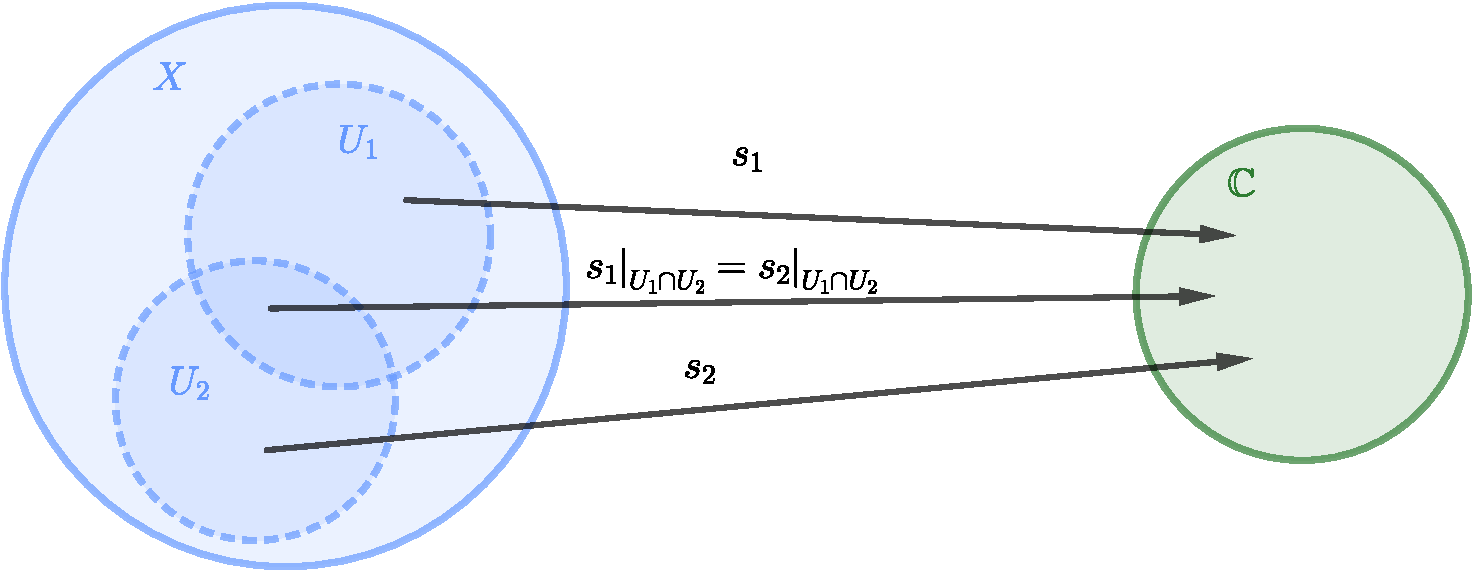
\includegraphics[scale=0.3]{Sheaf_condition.pdf}
    \end{figure}

\end{frame}
\begin{frame}
    \frametitle{Examples}

    Typical examples are rings of functions:
    \begin{itemize}
        \item $\Cont(-, \bbC)$
        \item $C^\infty(-, \bbC)$
    \end{itemize}
    \pause
    \medskip

    \medskip
    The constant functor $U \mapsto Y$ is \emph{not} a sheaf!

    Sheaf conditions imply $\mcF(\emptyset) = \{*\}$
\end{frame}

\begin{frame}
    \frametitle{Limits and Colimits}

    \begin{proposition}
        Limits and colimits of presheaves can be computed
        section-wise, i.e. the functor $\mcF \mapsto \mcF(U)$
        commutes with all limits and colimits.
    \end{proposition}

    \pause
    \begin{example}
        $(\mcF\times \mcG )(U) = \mcF(U) \times \mcG(U)$
    \end{example}

\end{frame}

\begin{frame}
    \frametitle{Sheafification}

    \begin{center}
        Can we do the same for sheaves?
    \end{center}
    \pause
    \begin{itemize}
        \item Limits: ok.
        \item Colimits: not always a sheaf.
    \end{itemize}
    There is a solution:
    \pause
    \begin{theorem}
        The fully faithful inclusion $\iota \colon \Sh(X) \injto \PSh(X)$
        admits an \emph{exact} left adjoint: \emph{sheafification}.
    \end{theorem}
    \begin{example}
        Sheafification of $U \mapsto Y$, is $U \mapsto \Cont(U, Y_{\text{discrete}})$.
    \end{example}

\end{frame}

\begin{frame}
    \frametitle{Abelian Sheaves}

    \begin{proposition}
        The category of abelian sheaves on a topological space $X$
        is abelian, and has enough injectives.
    \end{proposition}

    \begin{example}
        If $M$ is an injective object in $\Ab$, i.e. a divisible group,
        then for $x\in X$,
        \begin{equation*}
            U \mapsto
            \begin{cases}
                M     & x \in U    \\
                \{*\} & x \notin U
            \end{cases}
        \end{equation*}
        is an injective sheaf.
    \end{example}

\end{frame}

\begin{frame}
    \frametitle{Sheaf Cohomology}

    If
    \begin{equation*}
        \begin{tikzcd}[ampersand replacement=\&]
            0 \rar \& \mcF \rar \& \mcF' \rar \& \mcF'' \rar \& 0
        \end{tikzcd}
    \end{equation*}
    is exact, then globally we only get
    \begin{equation*}
        \begin{tikzcd}[ampersand replacement=\&]
            0 \rar \& \mcF(X) \rar \& \mcF'(X) \rar \& \mcF''(X)
        \end{tikzcd}
    \end{equation*}
    \pause
    $\leadsto$ Right derived functors $H^i(X, -)$ of $\mcF \mapsto \mcF(X)$
    \begin{definition}
        The sheaf cohomology of $X$ with coefficients $A$ is $H^i(X, \Cont(- , A))$.
    \end{definition}

\end{frame}

\begin{frame}
    \frametitle{Computing Homology}

    We have
    \begin{equation*}
        \begin{tikzcd}[ampersand replacement=\&, sep=small, cramped]
            0 \rar \& \Cont(-, \bbZ) \rar \& \Cont(-, \bbR) \rar
            \& \Cont(-, \bbR/\bbZ) \rar \& 0
        \end{tikzcd}
    \end{equation*}
    since every map $U\subseteq S^1 \to S^1$ can be
    lifted \emph{locally} to a map $U \to \bbR$.

    \medskip
    But, there is no global lift of $\id\colon S^1 \to S^1$
    to $S^1 \to \bbR$.
    So $H^1(S^1, \bbZ) \neq 0$.

    \medskip
    \pause
    \begin{proposition}
        If $X$ is a CW-complex:
        \begin{equation*}
            H^i_{\text{sheaf}}(X, \bbZ) = H^i_{\text{singular}}(X, \bbZ).
        \end{equation*}
    \end{proposition}

\end{frame}

\begin{frame}
    \frametitle{Sites}

    \begin{itemize}
        \item Need a slight abstraction of sheaves on a space.
        \item Want sheaves on categories, not just spaces.
        \item Crucial ingredient: coverings.
    \end{itemize}
    \medskip

    \pause
    $\leadsto$ Definition of a site $\approx $ ``Category + notion of coverings''.

\end{frame}

\begin{frame}
    \frametitle{Profinite sets}


    \begin{definition}
        A \emph{profinite set} is a compact, Hausdorff, totally disconnected space.
    \end{definition}
    \begin{example}
        A finite discrete space
    \end{example}
    \pause

    \begin{proposition}
        A limit of profinite sets is profinite.
        In particular, products of profinite sets
        are again profinite.
    \end{proposition}

\end{frame}

\begin{frame}
    \frametitle{Condensed Sets}

    \begin{definition}
        A \emph{condensed set}\onslide<2->{$^*$} is a sheaf on the site of profinite sets
        with coverings given by finite families of jointly surjective maps.
    \end{definition}
    \medskip
    \pause[3]
    \begin{proposition}
        Condensed abelian groups form an abelian category, and
        limits and colimits can be computed section-wise.
    \end{proposition}

    \pause

    For a topological space $X$, the associated condensed set $\underline{X}$
    is given by $\Cont(-,X)$.
\end{frame}

\begin{frame}
    \frametitle{The motivating problem}

    Recall that
    \begin{equation*}
        \id \colon \bbR_{\text{discrete}} \to \bbR_{\text{Euclidean}}
    \end{equation*}
    was both a monomorphism and an epimorphism but not an isomorphism.
    \pause

    \textbf{Claim}: As condensed abelian groups, the map:
    \begin{equation*}
        \underline{\id} \colon \underline{\bbR_{\text{discrete}}} \to \underline{\bbR_{\text{Euclidean}}}
    \end{equation*}
    is no longer an epimorphism.
\end{frame}
\begin{frame}
    \frametitle{The Cantor Set}
    Enough to show:
    \begin{equation*}
        \Cont(S, \bbR_{\text{discrete}}) \subsetneq \Cont(S, \bbR_{\text{Euclidean}})
    \end{equation*}
    for some profinite set $S$.

    \pause
    \medskip

    Let $S \subset \bbR_{\text{Euclidean}}$ be the cantor set.
    $ S \cong \prod_{n\in \bbN}\{0,1\}$,
    so $S$ is profinite.
    Hence:
    \begin{equation*}
        \Cont(S, \bbR_{\text{discrete}}) \subsetneq \Cont(S, \bbR_{\text{Euclidean}})
    \end{equation*}

    \begin{figure}
        \centering
        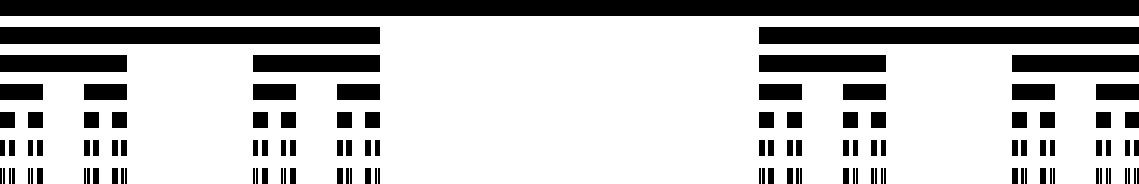
\includegraphics[scale=0.5]{Cantor_set_in_seven_iterations.pdf}
    \end{figure}

\end{frame}
\begin{frame}
    \frametitle{Condensed cohomology}

    For a condensed set $T$, let $\bbZ[T]$ be the sheafification
    of $S \mapsto \bbZ[T(S)]$.
    \begin{definition}
        The cohomology of $S$ with coefficients $A$ is
        \begin{equation*}
            H^i (S, A) = \Ext^i(\bbZ[\underline{S}], \underline{A})
        \end{equation*}
    \end{definition}

    \pause
    \begin{theorem}[\cite{Sch2019LecturesCM}, Theorem 3.2]
        Let $S$ be a compact Hausdorff space. Then
        \begin{equation*}
            H^i_{\text{cond}}(S, A) \cong H^i_{\text{sheaf}}(S, A)
        \end{equation*}
    \end{theorem}

\end{frame}

\bibliographystyle{alpha}
\begin{frame}{References}
    \nocite{Sch2019LecturesCM}
    \nocite{Apa2021condensed}
    \nocite{stacks-project}
    \nocite{Sch2020MasterClass}
    \bibliography{references.bib}
\end{frame}
\end{document}
